% ********************************************************************
% *                  Format for IMVIP 2019  papers,                  *
% *         based on the IMVIP 2001, 2006, 2014-2018 templates       *
% ********************************************************************
\documentclass[a4paper,11pt]{article}



\setlength{\topmargin}{-0.5cm}
\setlength{\headsep}{.5cm}
%\setlength{\footskip}{1.0cm}
\setlength{\textheight}{24cm}
\setlength{\textwidth}{17cm}
\setlength{\evensidemargin}{-.5cm}
\setlength{\oddsidemargin}{-.5cm}



\usepackage{fourier}
\usepackage{color}
 \usepackage{graphicx}
\usepackage{url}
\usepackage[affil-it]{authblk}
\usepackage{amsmath}
\usepackage{wrapfig}
\usepackage{xspace}

\usepackage[T1]{fontenc}
\usepackage{times}


\pagestyle{empty}

%%%%
\begin{document}

\title{Author Instructions for IMVIP 2019}

\author{Michael McDonagh}
\affil{Anonymous Affiliation}
\date{}
\maketitle
\thispagestyle{empty}



\begin{abstract}
This study explores the development of a deep learning system to classify 19 different types of food. Recognising food from images is a difficult task because many dishes look very similar and the way a meal is plated can vary significantly. This research compares two main methods: a custom-built Convolutional Neural Network (CNN) and a Transfer Learning approach that uses a pre-trained model as its foundation.
\end{abstract}
\textbf{Keywords:} Imaging, Image Processing, Machine Vision, etc. (Maximum five)



%%%%%%%%%%%%%%%%%%%%%%
\section{Introduction}
\begin{wrapfigure}{r}{0.5\textwidth}
  \vspace{-20pt}
  \begin{center}
    \includegraphics[width=0.4\textwidth]{DIT_Grangegorman.png}
\end{center}
\vspace{-20pt}
  \caption{Introduction Banner.}
  \vspace{-0pt}
\end{wrapfigure}
%%%%%%%%%%%%%%%%%%%%%%
Initial attempts with a custom model resulted in clear underfitting, where the accuracy was no better than random guessing at 5.2\%. By improving the model structure, specifically by using double convolutional blocks, increasing the number of filters to 128, adding Dropout Layers to prevent over-reliance on specific features, the custom model eventually achieved a stable validation accuracy of 65\%. To try and improve further, a two-phase transfer learning strategy was used. THis involved an initial phase where the base model was frozen, followed by a fine-tuning phase to adapt the weights to this specific food dataset.
%%

\section{Data and Pre-Processing}
Sed ut perspiciatis, unde omnis iste natus error sit voluptatem accusantium doloremque laudantium, totam rem aperiam eaque ipsa, quae ab illo inventore veritatis et quasi architecto beatae vitae dicta sunt, explicabo. Nemo enim ipsam voluptatem, quia voluptas sit, aspernatur aut odit aut fugit, sed quia consequuntur magni dolores eos, qui ratione voluptatem sequi nesciunt, neque porro quisquam est, qui dolorem ipsum, quia dolor sit amet consectetur adipisci[ng] velit, sed quia non numquam [do] eius modi tempora inci[di]dunt, ut labore et dolore magnam aliquam quaerat voluptatem. Ut enim ad minima veniam, quis nostrum exercitationem ullam corporis suscipit laboriosam, nisi ut aliquid ex ea commodi consequatur? Quis autem vel eum iure reprehenderit, qui in ea voluptate velit esse, quam nihil molestiae consequatur, vel illum, qui dolorem eum fugiat, quo voluptas nulla pariatur?

\subsection{Dataset Description}

Sed ut perspiciatis, unde omnis iste natus error sit voluptatem accusantium doloremque laudantium, totam rem aperiam eaque ipsa, quae ab illo inventore veritatis et quasi architecto beatae vitae dicta sunt, explicabo. Nemo enim ipsam voluptatem, quia voluptas sit, aspernatur aut odit aut fugit, sed quia consequuntur magni dolores eos, qui ratione voluptatem sequi nesciunt, neque porro quisquam est, qui dolorem ipsum, quia dolor sit amet consectetur adipisci[ng] velit, sed quia non numquam [do] eius modi tempora inci[di]dunt, ut labore et dolore magnam aliquam quaerat voluptatem. Ut enim ad minima veniam, quis nostrum exercitationem ullam corporis suscipit laboriosam, nisi ut aliquid ex ea commodi consequatur? Quis autem vel eum iure reprehenderit, qui in ea voluptate velit esse, quam nihil molestiae consequatur, vel illum, qui dolorem eum fugiat, quo voluptas nulla pariatur?

\subsubsection{Exploratory Analysis}

Sed ut perspiciatis, unde omnis iste natus error sit voluptatem accusantium doloremque laudantium, totam rem aperiam eaque ipsa, quae ab illo inventore veritatis et quasi architecto beatae vitae dicta sunt, explicabo. Nemo enim ipsam voluptatem, quia voluptas sit, aspernatur aut odit aut fugit, sed quia consequuntur magni dolores eos, qui ratione voluptatem sequi nesciunt, neque porro quisquam est, qui dolorem ipsum, quia dolor sit amet consectetur adipisci[ng] velit, sed quia non numquam [do] eius modi tempora inci[di]dunt, ut labore et dolore magnam aliquam quaerat voluptatem. Ut enim ad minima veniam, quis nostrum exercitationem ullam corporis suscipit laboriosam, nisi ut aliquid ex ea commodi consequatur? Quis autem vel eum iure reprehenderit, qui in ea voluptate velit esse, quam nihil molestiae consequatur, vel illum, qui dolorem eum fugiat, quo voluptas nulla pariatur?


\subsubsection{Preprocessing and Splits}

Sed ut perspiciatis, unde omnis iste natus error sit voluptatem accusantium doloremque laudantium, totam rem aperiam eaque ipsa, quae ab illo inventore veritatis et quasi architecto beatae vitae dicta sunt, explicabo. Nemo enim ipsam voluptatem, quia voluptas sit, aspernatur aut odit aut fugit, sed quia consequuntur magni dolores eos, qui ratione voluptatem sequi nesciunt, neque porro quisquam est, qui dolorem ipsum, quia dolor sit amet consectetur adipisci[ng] velit, sed quia non numquam [do] eius modi tempora inci[di]dunt, ut labore et dolore magnam aliquam quaerat voluptatem. Ut enim ad minima veniam, quis nostrum exercitationem ullam corporis suscipit laboriosam, nisi ut aliquid ex ea commodi consequatur? Quis autem vel eum iure reprehenderit, qui in ea voluptate velit esse, quam nihil molestiae consequatur, vel illum, qui dolorem eum fugiat, quo voluptas nulla pariatur?


%%
\subsection{Experiments}

Sed ut perspiciatis, unde omnis iste natus error sit voluptatem accusantium doloremque laudantium, totam rem aperiam eaque ipsa, quae ab illo inventore veritatis et quasi architecto beatae vitae dicta sunt, explicabo. Nemo enim ipsam voluptatem, quia voluptas sit, aspernatur aut odit aut fugit, sed quia consequuntur magni dolores eos, qui ratione voluptatem sequi nesciunt, neque porro quisquam est, qui dolorem ipsum, quia dolor sit amet consectetur adipisci[ng] velit, sed quia non numquam [do] eius modi tempora inci[di]dunt, ut labore et dolore magnam aliquam quaerat voluptatem. Ut enim ad minima veniam, quis nostrum exercitationem ullam corporis suscipit laboriosam, nisi ut aliquid ex ea commodi consequatur? Quis autem vel eum iure reprehenderit, qui in ea voluptate velit esse, quam nihil molestiae consequatur, vel illum, qui dolorem eum fugiat, quo voluptas nulla pariatur?

\subsection{CNN From Scratch}

The first CNN model, \textbf{Model V1} I had developed was configured with two convolutional blocks for feature extract and a single MaxPooling2D for downsampling after each. With the initial baseline model I had observed that it had suffered from extreme overfitting, having a training accuracy of 99\% while the validation accuracy was stuck around 20\%. This clear gap showcases that the model was memorising the training data and could not generalise on new unseen data. 

The next iteration with \textbf{Model V2} focused on combatting the overfitting problem by introducing a total of three convolutional blocks, doubling each layer to 2 instead of 1 so it can focuse on fidning more features, dense increased to 256, and also introducing Dropout at `0.5' as this would force the network to not rely on any specific node. The model resulted in val accuracy at 0.055\% followed by train accuracy at 0.053\%, showcasing the model moving in the opposite direction, from overfitting, to underfitting. 

Finding the perfect balance where the model can learn patterns and generalise on new unseen data is key, so in \textbf{Model V3}, I had scaed back to 2 convolutional blocks with each containing batch normalisation to prevent numbers becoming too large as they move through the layers, and then the MaxPooling2D. GlobalAveragePooling2D was also used to reduce the number of parameters down from `8,680,755` to `41,299`. This model iteration showed the most progress so far, where the training accuracy is smoothly increasing and loss is smoothly decreasing. Furthermore, the validation loss is decreasing with some stagnation, and accuracy is increasing with that same stagnation but keeping close in line with the respective train lines.

Moving onto \textbf{Model V4}, we introduce image augmentation, to modify the dataset images to help improve generalisation. The augmentation added were to flip, rotate and zoom the dataset images. This improved the stability of the training loss but introduced significant volatility in the validation metrics. The final validaiton accuracy of 38\% suggests that while the model is learning general features, it remains sensitive to extreme image transformations.

The models \textbf{V5} and \textbf{V6} respectively, focused on inreasing the convolutional layer filters to help detect more complex semantic features, with \textbf{V5} having a max `256` filter and \textbf{V6} `1024` filter, further pushing the dense layer towards `2048`. \textbf{V6} had been able to increase the validation accurcy to ~67\% as a result.

In \textbf{Model V7}, the architecture was further deepened to include a 512-filter stage while significantly increasing the Dropout rate to $0.6$ \ref{tab:model_performance} and reducing the learning rate to $0.0001$ \ref{tab:model_performance}. The objective was to prioritise stability and prevent the volatility observed in earlier versions. While the training curves appeared smoother (as seen in Figure \ref{fig:cnn_comparison}), the model achieved a final validation accuracy of approximately 60\%, failing to surpass the performance of the shallower V6 architecture\ref{tab:model_performance}. 

The final iteration, \textbf{Model V8}, took inspiration from the high-capacity filter banks of V6 but extended the training duration to 100 epochs and expanded the dense layer to 2048 units. Despite the additional training time and increased model capacity, the validation accuracy plateaued early and eventually began to diverge, as seen in the widening gap between the training and validation loss curves in Figure \ref{fig:cnn_comparison}.

Ultimately, \textbf{Model V6} was identified as the superior architecture developed from scratch. It provided the optimal balance of depth and width, achieving a peak validation accuracy of $\approx$ 67\% \ref{tab:model_performance} without the severe overfitting seen in V8 or the over-regularisation of V7. This model served as the final benchmark for our custom-built architectures before transitioning to transfer learning techniques.

\begin{figure}[h!]
    \centering
    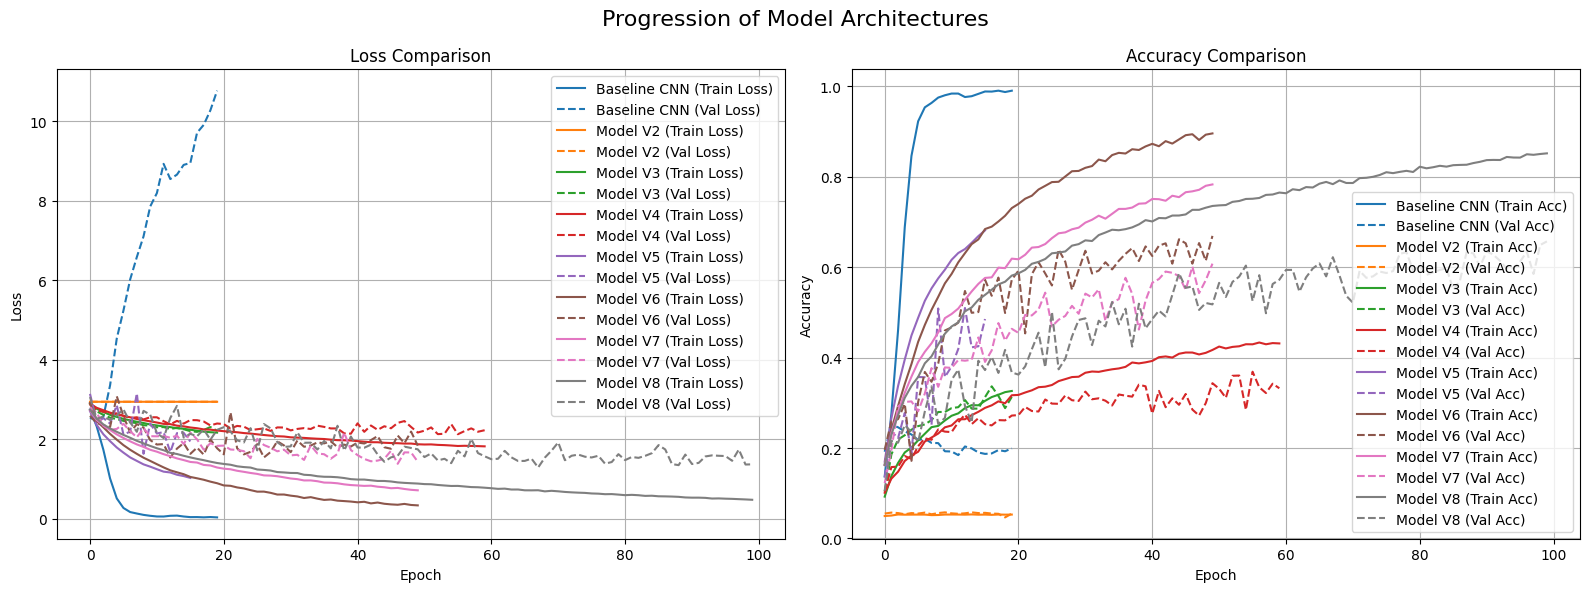
\includegraphics[width=0.8\textwidth]{images/compare-cnn-scratch.png}
    \caption{Performance Comparison of CNN Architectures from Scratch}
    \label{fig:cnn_comparison}
\end{figure}

\begin{table}[h]
\centering
\caption{Model Performance Comparison Tracker. Improvement metric is based on comparison with the Baseline CNN Model}
\label{tab:model_performance}
\begin{tabular}{@{}lccccr@{}}
\toprule
\textbf{Model Version} & \textbf{Time (s)} & \textbf{Final Train Acc} & \textbf{Final Val Acc} & \textbf{Final Val Loss} & \textbf{Improvement (\%)} \\ \midrule
Baseline CNN           & 1029.10           & 0.9899                   & 0.1992                 & 10.7718                 & 0.00                      \\
Model V2               & 1029.10           & 0.0529                   & 0.0551                 & 2.9453                  & -14.41                    \\
Model V3               & 1029.10           & 0.3261                   & 0.3130                 & 2.2151                  & 11.38                     \\
Model V4               & 1029.10           & 0.4312                   & 0.3321                 & 2.2290                  & 13.29                     \\
Model V5               & 1029.10           & 0.6811                   & 0.4852                 & 1.9460                  & 28.60                     \\
\textbf{Model V6}              & 1029.10           & 0.8955                   & 0.6690                 & 1.8402                  & 46.98                     \\
Model V7               & 2033.53           & 0.8514                   & 0.6568                 & 1.3706                  & 45.76                     \\
Model V7     & 2033.53           & 0.8514                   & 0.6568                 & 1.3706                  & 45.76                     \\ \bottomrule
\end{tabular}
\end{table}

\subsection{Transfer Learning}

Sed ut perspiciatis, unde omnis iste natus error sit voluptatem accusantium doloremque laudantium, totam rem aperiam eaque ipsa, quae ab illo inventore veritatis et quasi architecto beatae vitae dicta sunt, explicabo. Nemo enim ipsam voluptatem, quia voluptas sit, aspernatur aut odit aut fugit, sed quia consequuntur magni dolores eos, qui ratione voluptatem sequi nesciunt, neque porro quisquam est, qui dolorem ipsum, quia dolor sit amet consectetur adipisci[ng] velit, sed quia non numquam [do] eius modi tempora inci[di]dunt, ut labore et dolore magnam aliquam quaerat voluptatem. Ut enim ad minima veniam, quis nostrum exercitationem ullam corporis suscipit laboriosam, nisi ut aliquid ex ea commodi consequatur? Quis autem vel eum iure reprehenderit, qui in ea voluptate velit esse, quam nihil molestiae consequatur, vel illum, qui dolorem eum fugiat, quo voluptas nulla pariatur?

\subsection{Results and Comparison}
Sed ut perspiciatis, unde omnis iste natus error sit voluptatem accusantium doloremque laudantium, totam rem aperiam eaque ipsa, quae ab illo inventore veritatis et quasi architecto beatae vitae dicta sunt, explicabo. Nemo enim ipsam voluptatem, quia voluptas sit, aspernatur aut odit aut fugit, sed quia consequuntur magni dolores eos, qui ratione voluptatem sequi nesciunt, neque porro quisquam est, qui dolorem ipsum, quia dolor sit amet consectetur adipisci[ng] velit, sed quia non numquam [do] eius modi tempora inci[di]dunt, ut labore et dolore magnam aliquam quaerat voluptatem. Ut enim ad minima veniam, quis nostrum exercitationem ullam corporis suscipit laboriosam, nisi ut aliquid ex ea commodi consequatur? Quis autem vel eum iure reprehenderit, qui in ea voluptate velit esse, quam nihil molestiae consequatur, vel illum, qui dolorem eum fugiat, quo voluptas nulla pariatur?
\subsection{Real-World Test}
Sed ut perspiciatis, unde omnis iste natus error sit voluptatem accusantium doloremque laudantium, totam rem aperiam eaque ipsa, quae ab illo inventore veritatis et quasi architecto beatae vitae dicta sunt, explicabo. Nemo enim ipsam voluptatem, quia voluptas sit, aspernatur aut odit aut fugit, sed quia consequuntur magni dolores eos, qui ratione voluptatem sequi nesciunt, neque porro quisquam est, qui dolorem ipsum, quia dolor sit amet consectetur adipisci[ng] velit, sed quia non numquam [do] eius modi tempora inci[di]dunt, ut labore et dolore magnam aliquam quaerat voluptatem. Ut enim ad minima veniam, quis nostrum exercitationem ullam corporis suscipit laboriosam, nisi ut aliquid ex ea commodi consequatur? Quis autem vel eum iure reprehenderit, qui in ea voluptate velit esse, quam nihil molestiae consequatur, vel illum, qui dolorem eum fugiat, quo voluptas nulla pariatur?
\subsection{Conclusion}
Sed ut perspiciatis, unde omnis iste natus error sit voluptatem accusantium doloremque laudantium, totam rem aperiam eaque ipsa, quae ab illo inventore veritatis et quasi architecto beatae vitae dicta sunt, explicabo. Nemo enim ipsam voluptatem, quia voluptas sit, aspernatur aut odit aut fugit, sed quia consequuntur magni dolores eos, qui ratione voluptatem sequi nesciunt, neque porro quisquam est, qui dolorem ipsum, quia dolor sit amet consectetur adipisci[ng] velit, sed quia non numquam [do] eius modi tempora inci[di]dunt, ut labore et dolore magnam aliquam quaerat voluptatem. Ut enim ad minima veniam, quis nostrum exercitationem ullam corporis suscipit laboriosam, nisi ut aliquid ex ea commodi consequatur? Quis autem vel eum iure reprehenderit, qui in ea voluptate velit esse, quam nihil molestiae consequatur, vel illum, qui dolorem eum fugiat, quo voluptas nulla pariatur?

\subsection{Bibliographic references}
References in a bib file format (e.g. imvip2019.bib given in the template) can be inserted using bibtex along with
\LaTeX\xspace/pdflatex (e.g.  \cite{hartley} or  \cite{jain, goodfellow}). 


\bibliographystyle{apalike}

\bibliography{imvip}


\end{document}

